\documentclass{ximera}

\newcommand{\RR}{\mathbb R}
\renewcommand{\d}{\,d}
\newcommand{\dd}[2][]{\frac{d #1}{d #2}}
\renewcommand{\l}{\ell}
\newcommand{\ddx}{\frac{d}{dx}}
\newcommand{\dfn}{\textbf}
\newcommand{\eval}[1]{\bigg[ #1 \bigg]}


\begin{document}



\begin{problem}
Let $\vec{p}(t)$ be the vector valued function shown below:
\begin{image}
    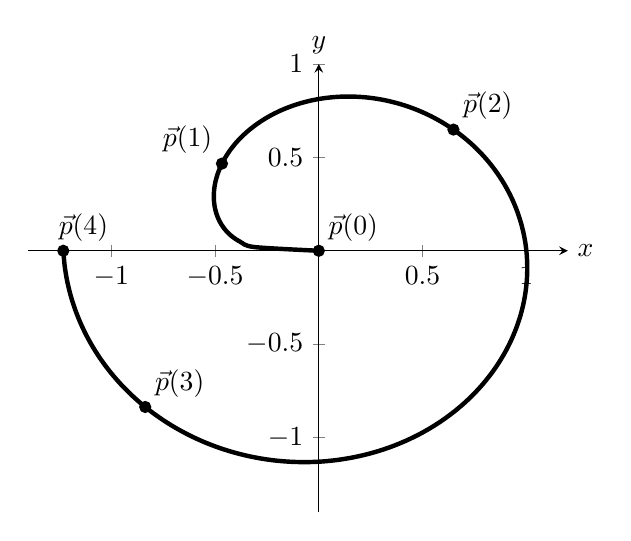
\begin{tikzpicture}
      \begin{axis}[
          xmin=-1.4, xmax=1.2, ymin =-1.4, ymax = 1,
          axis lines=center,  
          xlabel=$x$,  
          ylabel=$y$,  
          every axis y label/.style={at=(current axis.above origin),anchor=south},  
          every axis x label/.style={at=(current axis.right of origin),anchor=west}
        ]
        \addplot [black,ultra thick,domain=0:360,smooth,samples=100] ({-((x/180)^(.3))*cos(x)},{((x/180)^.3)*sin(x)});
        \node[above right,black] at (axis cs: 0,0) {$\vec{p}(0)$};
        \node[above right,black] at (axis cs: -1.3,0) {$\vec{p}(4)$};
        \node[above right,black] at (axis cs: {-((135/180)^(.3))*cos(135)},{((135/180)^.3)*sin(135)}) {$\vec{p}(2)$};
        \node[above left,black] at (axis cs: {-((45/180)^(.3))*cos(45)},{((45/180)^.3)*sin(45)}) {$\vec{p}(1)$};
        \node[above right,black] at (axis cs: {-((315/180)^(.3))*cos(315)},{((315/180)^.3)*sin(315)}) {$\vec{p}(3)$};
        
        \addplot[color=black,fill=black,only marks,mark=*] coordinates{(-{((45/180)^(.3))*cos(45)},{((45/180)^.3)*sin(45)})};
        \addplot[color=black,fill=black,only marks,mark=*] coordinates{(-{((135/180)^(.3))*cos(135)},{((135/180)^.3)*sin(135)})};
        \addplot[color=black,fill=black,only marks,mark=*] coordinates{(-{((315/180)^(.3))*cos(315)},{((315/180)^.3)*sin(315)})};
        \addplot[color=black,fill=black,only marks,mark=*] coordinates{(-{((360/180)^(.3))*cos(360)},{((360/180)^.3)*sin(360)})};
        \addplot[color=black,fill=black,only marks,mark=*] coordinates{(0,0)};
        
      \end{axis}
    \end{tikzpicture}
\end{image}
\begin{itemize}
  \item \textbf{Sketch a tangent vector} for $\vec{p}$ at $t=1$ on the graph above.
  \item Let $\utan$ be the unit tangent vector for $\vec{p}$. \textbf{Sketch a vector in the same direction} as
    $\utan'(2)$ at $\vec{p}(2)$.
  \item Suppose that $\utan(t) = \vector{x(t),y(t)}$. \textbf{Sketch a vector
    in the same direction} as $\vector{y(3),-x(3)}$ at $\vec{p}(3)$.
\end{itemize}

\begin{prompt}
  \begin{multipleChoice}
    \choice[correct]{I've drawn these vectors.}
  \end{multipleChoice}
  \begin{feedback}[correct]
\begin{image}
    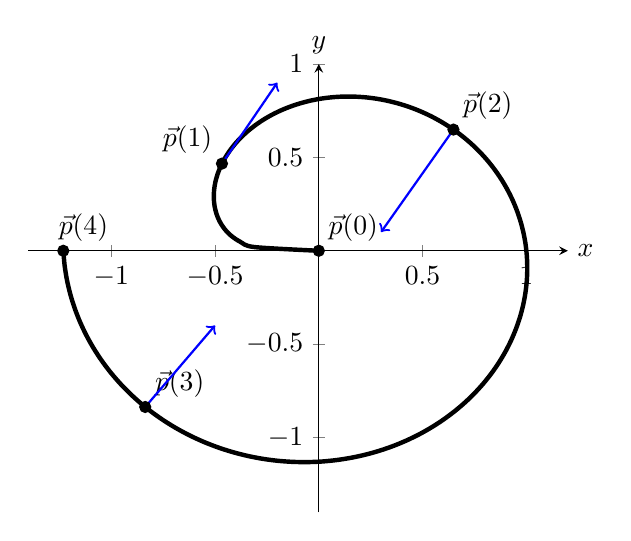
\begin{tikzpicture}
      \begin{axis}[
          xmin=-1.4, xmax=1.2, ymin =-1.4, ymax = 1,
          axis lines=center,  
          xlabel=$x$,  
          ylabel=$y$,  
          every axis y label/.style={at=(current axis.above origin),anchor=south},  
          every axis x label/.style={at=(current axis.right of origin),anchor=west},
          clip=false
        ]
        \addplot [black,ultra thick,domain=0:360,smooth,samples=100] ({-((x/180)^(.3))*cos(x)},{((x/180)^.3)*sin(x)});
        \node[above right,black] at (axis cs: 0,0) {$\vec{p}(0)$};
        \node[above right,black] at (axis cs: -1.3,0) {$\vec{p}(4)$};
        \node[above right,black] at (axis cs: {-((135/180)^(.3))*cos(135)},{((135/180)^.3)*sin(135)}) {$\vec{p}(2)$};
        \node[above left,black] at (axis cs: {-((45/180)^(.3))*cos(45)},{((45/180)^.3)*sin(45)}) {$\vec{p}(1)$};
        \node[above right,black] at (axis cs: {-((315/180)^(.3))*cos(315)},{((315/180)^.3)*sin(315)}) {$\vec{p}(3)$};
        
        \addplot[color=black,fill=black,only marks,mark=*] coordinates{(-{((45/180)^(.3))*cos(45)},{((45/180)^.3)*sin(45)})};
        \addplot[color=black,fill=black,only marks,mark=*] coordinates{(-{((135/180)^(.3))*cos(135)},{((135/180)^.3)*sin(135)})};
        \addplot[color=black,fill=black,only marks,mark=*] coordinates{(-{((315/180)^(.3))*cos(315)},{((315/180)^.3)*sin(315)})};
        \addplot[color=black,fill=black,only marks,mark=*] coordinates{(-{((360/180)^(.3))*cos(360)},{((360/180)^.3)*sin(360)})};
        \addplot[color=black,fill=black,only marks,mark=*] coordinates{(0,0)};

        \addplot[blue,->,thick] coordinates{(-{((45/180)^(.3))*cos(45)},{((45/180)^.3)*sin(45)}) (-.2,.9)};
        \addplot[blue,->,thick] coordinates{(-{((135/180)^(.3))*cos(135)},{((135/180)^.3)*sin(135)})
          (.3,.1)};
        \addplot[blue,->,thick] coordinates{(-{((315/180)^(.3))*cos(315)},{((315/180)^.3)*sin(315)}) (-.5,-.4)};
      \end{axis}
    \end{tikzpicture}
\end{image}
  \end{feedback}
\end{prompt}



\end{problem}

\hrule

\textbf{For problems 17--18,} let $\vec{p}(t) = \vector{t,t^2,t^3}$

\begin{problem}
  Find a vector-valued function that draws the tangent line for the
  curve drawn by $\vec{p}$ at $t=a$.
  \begin{prompt}
  \[
  \vecl(t) = \vector{\answer{a+t},\answer{a^2+2at},\answer{a^3 + 3a^2t}}
  \]
  \end{prompt}

  \vfill
  
\end{problem}


\begin{problem}
  Letting $\vecl$ be the vector-valued function that draws the \textbf{tangent
  line} for the curve drawn by $\vec{p}$ at $t=2$, find the $(x,y,z)$
  coordinates for where $\vecl$ \textbf{intersects} the $(x,y)$-plane.
  \begin{prompt}
    \[
    (x,y,z) = \left(\answer{2-8/12},\answer{4-32/12},\answer{0}\right)
    \]
  \end{prompt}

  \vfill
  
\end{problem}

\end{document}
